\documentclass[conference]{IEEEtran}
\IEEEoverridecommandlockouts
% The preceding line is only needed to identify funding in the first footnote. If that is unneeded, please comment it out.
\usepackage{cite}
\usepackage{amsmath,amssymb,amsfonts}
\usepackage{graphicx}
\usepackage{textcomp}
\usepackage{xcolor}
\usepackage{hyperref}
\usepackage[utf8]{inputenc}
\def\BibTeX{{\rm B\kern-.05em{\sc i\kern-.025em b}\kern-.08em
    T\kern-.1667em\lower.7ex\hbox{E}\kern-.125emX}}
\begin{document}

\title{Classificação de textos com Natural Language Processing em Python\\
{\footnotesize \textsuperscript{*}Utilização de machine learning para classificação de relatos policiais em suas naturezas}
}


\author{\IEEEauthorblockN{Fabiano Araujo}
\IEEEauthorblockA{\textit{Universidade La Salle} \\
\textit{UNILASALLE}\\
Canoas, Brasil \\}
}

\maketitle

\begin{abstract}
A NoSQL engine provides faster and less reliable way to store and retrieve data. Redis is a software developed using the key-value model to provide that simple yet ubiquitous way of data storage.
\end{abstract}

\begin{IEEEkeywords}
Machine Learning, NLP, classification, python.
\end{IEEEkeywords}

\section{Introdução}

\section{Referencial Teórico}

A utilização de \textit{machine learning} \cite{Sebastiani:2002:MLA:505282.505283} 

TODO: crescente uso de machine learning

Entre diversos modelos matemáticos que aproximam a precisão de dois conjuntos de dados: de treinamento e de testes, existem parâmetros a serem adaptados para cada natureza de dados e para cada objetivo. O uso de \textit{machine learning} ainda que mais comum que anos antigos devido à melhor capacidade de hardware, não exime a necessidade de um hardware considerável, sendo diretamente relacionado para o desenvolvimento do modelo inicial. 

Divide-se em dois tipos de aprendizados de máquina, entre não supervisionados e supervisionados, cujo detalhes estão dispostos mais a frente. Para a definição de um modelo ótimo de \textit{machine learning} ainda existem passos anteriores do que a própria execução da máquina. 

É comum a expressão que a maior parte do tempo dos cientistas de dados nos estágios iniciais de uma implementação de um \textit{machine learning} é dedicado para o entendimento do problema e nas necessidades de aumentar a correlação dos valores, no pré-processamento dos dados, nos parâmetros de modelo que influenciam na precisão do modelo.

Os tipos de resultados também manipulam a forma de implementação dos algoritmos, visto que podem ser divididos principalmente em modelos regressores ou modelos classificadores. O acervo aberto de datasets conhecido com UCI Machine Learning Repository, criado inicialmente como um FTP em 1987 \cite{uciabout}, demonstra que ao longo dos anos é mais comum a publicação de datasets em classificação.

Os tipos de algoritmos também variam para cada tipo de dado utilizado, como uso de CNN (\textit{Convolucionary Neural Network}) para identificação de imagens ou ANN (\textit{Artificial Neural Network}) para aprendizado profundo de grande quantidade de dados com maior precisão de retorno, ou mesmo NLP (\textit{Natural Language Processing}) que se compromete a separação dos dados agregando pesos aos valores entre palavras obtidas e o resultado esperado.

A utilização de classificação de textos teve início na década de 60, mas apenas na década de 90 pode ser efetivamente utilizado e sofreu maior avanço de pesquisa devida a maior capacidade de hardware \cite{Sebastiani:2002:MLA:505282.505283}. Até a década de 80, a classificação de textos era dependente de um engenheiro de conhecimento, em sua tradução livre a partir da ação \textit{knowledge engineering} \cite{Sebastiani:2002:MLA:505282.505283}. 

Para que tanto o resultado da implementação como os passos do pré-processamento utilizado possam ser entendidos, é necessário conceituar corretamente a vasta possibilidade de técnicas e metodologias disponíveis para utilização de \textit{machine learning}. Este conjunto de técnicas e análise prévia de dados recebe o nome de Ciência de dados.

\subsection{Ciência de dados}

A frequência com que o nome ciência de dados é apresentada por diversos meios de leitura e disseminação de informação, demonstra quase um descaso pelo real e complexo ambiente de assuntos e tópicos de pesquisa que abrangem a ciência de dados. 

A ciência de dados é, na verdade, uma união de diversos assuntos, entre eles dados digitais, computação e matemática. Os três assuntos podem ser correlacionados entre si e quando agrupadas as ações, técnicas ou conhecimentos de pesquisa obtidos em cada uma das áreas, compõem-se o que se chama de ciência de dados, como mostra a figura 1, representando as três áreas pelo diagrama de Venn. \cite{datasciencecathy}

\begin{figure}[h]
\centerline{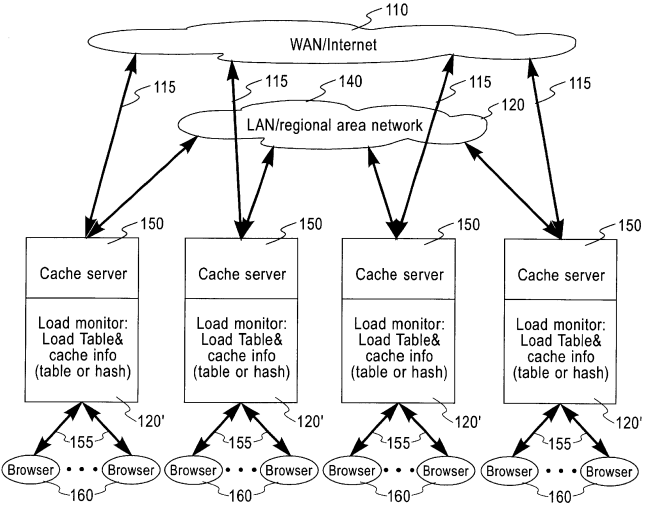
\includegraphics[width=0.5\linewidth]{figura1.png}}
\caption{Diferentes campos de pesquisa compõe a ciência de dados \cite{tds:barber}}
\label{fig}
\end{figure}

Segundo Mike Driscoll \cite{datasciencecathy}, em sua tradução: "Ciência de dados é a engenharia civil dos dados". Em consequência do efeito chamado \textit{datafication}, que é a absorção de informações em dados de diferentes ambientes e comportamentos, surge a necessidade de entender qual o comportamento dos dados. 

A finalidade deste artigo não é definir ciência de dados de uma forma simples, existe extensa discussão na área acadêmia e na industria que peca na definição dos termos e nas áreas de aplicação para que possam ser gerados limites entre os assuntos ou a definição de assuntos mínimos.

\subsection{Machine Learning}

\textit{Machine Learning} é um campo de pesquisa dentro da área de inteligência artificial que tem como premissa utilizar modelos matemáticos para prever valores. A habilidade de prever valores depende da capacidade de aprender padrões com base nos dados providos ao algoritmo e se segmentam em aprendizagem por reforço, supervisionado ou não supervisionado.

Aprendizado de máquina não supervisionado é utilizado quando os dados a serem utilizados não possuem uma classificação clara ou não podem ser agrupados visualmente. Estes algoritmos tendem a identificar subgrupos, ação chamada na literatura estrangeira de \textit{clustering}. Tal ação permite o analista a compreensão de comportamento \cite{pythonmachinelearning}.

Outro tipo de aprendizado de máquina é o chamado por reforço. Neste tipo, alguma informação é proposta para o modelo, porém o mesmo explora o ambiente em que se encontra e opta pelos melhores valores a partir de um mecanismo de recompensa\cite{pythonmachinelearning}. São comuns as aplicações de jogos digitais que treinam inteligência artificial para melhorara os chamados \textit{bots}, personagens controlados por computador inseridos no contexto competitivo ou cooperativo. O uso de \textit{Artificial Neural Network}, ANN, é um exemplo de aprendizado por reforço.

Por último, o aprendizado supervisionado remete a obtenção de dados previamente corretos que serão utilizados para demonstrar ao algoritmo os resultados esperados. Este tipo de aprendizado é segmentado ainda em aplicações de modelos de regressão ou de classificação.

Modelos de regressão têm o objetivo de retornar a predição de valores contínuos, como valores de salários ou temperaturas. Modelos de classificação têm o objetivo de classificar o dado novo com os grupos pré-definidos pelos dados fornecidos no processo de aprendizagem \cite{pythonmachinelearning}.

É fundamental observar que o processo de construção de uma máquina de aprendizado faz parte de um processo maior, conhecido pela sigla OSEMN (\textit{Obtain, Scrub, Explore, Model iNterpret} \cite{pythondatascience} demonstrado na figura 3. A utilização de algoritmos de aprendizagem ficam melhor alocados no passo \textit{Model}, visto que o mesmo trata da modelagem de dados. Há ainda a necessidade de visualizar os dados para garantir que o aprendizado está em um estado ótimo de precisão, cujo o mesmo pode gerar uma nova iteração desde o processo de captura.

Na literatura estrangeira, a fonte de onde os dados serão lidos é conhecido como \textit{dataset} e normalmente são representados por uma relação linhas e colunas. Cada linha do \textit{dataset} é conhecido como \textit{observation} e cada coluna, as variáveis, são chamadas de \textit{features}.

Uma das formas que algorítimos de \textit{Machine Learning} funcionam é utilizando de variáveis que influenciam diretamente no resultado, chamadas de variáveis dependentes, ou \textit{dependent variables}. A variável a que ser obter nos métodos regressores ou classificadores possui valor cujo é definido pelo conjunto combinado das variáveis dependentes e é chamada de variável independente, ou, \textit{independent variable}. 

Independente de qual algoritmo ou tipo de aprendizado será selecionado, existem passos anteriores à construção do código de \textit{Machine Learning} conhecido como pré-processamento. 

Dados obtidos diretamente de suas fontes dificilmente possuem todas as informações necessárias para gerar o aprendizado de máquina necessário para obter uma determinada precisão. Mais, existem diversas combinações de valores que podem não ser notórias à quem extraiu os dados ou, por maior que seja o conhecimento sobre o domínio dos dados, é incomparável a capacidade de identificação de correlação entre a máquina e o ser humano.

Durante o pré-processamento é possível identificar algumas técnicas adotadas para melhorar a precisão do aprendizado de máquina, visando o tratamento dos dados antes de serem inseridos no processo de treinamento, entre eles: \textit{feature scaling}, \textit{label encoding} e \textit{data cleaning}.

\textit{Feature scaling} trata-se da técnica de reduzir a discrepância entre mínimos e máximos de uma data \textit{feature}, onde os valores utilizados serão reestabelecidos com a grandeza equivalente onde o mínimo dos valores começaria de zero e por isto permitindo que o desempenho de precisão do algoritmo de aprendizagem seja maior, visto que os dados estão melhor distribuídos \cite{pythonmachinelearning}.

\textit{Label encoding} é a técnica de transcrever dados categóricos de modo não associar valores sequenciais aos mesmos para tornar a solução do algorítimos de aprendizagem tendenciosa pelo entendimento da grandeza de um valor sobre o outro. 

\begin{figure}[h]
\centerline{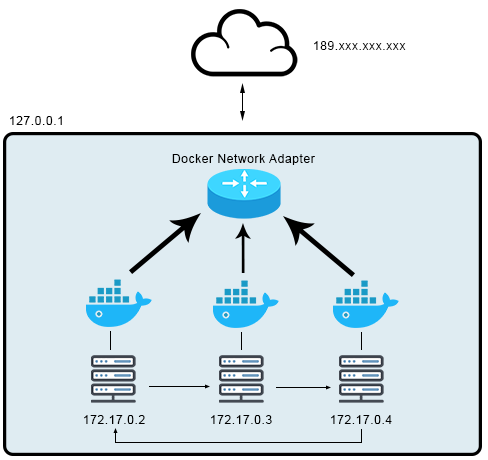
\includegraphics[width=1\linewidth]{figura3.png}}
\caption{Fluxo de aprendizado supervisionado \cite{pythonmachinelearning}}
\label{fig}
\end{figure}


A exemplo, dado um \textit{dataset} com algumas \textit{observations} onde uma delas é cor, e os dados possuem valores entre azul, verde ou vermelho, é sugestível tornar cada cor um valor inteiro sequencial, como azul ser representado por 1, verde por 2 e vermelho por 3. Porém na execução do treinamento do algoritmo de \textit{Machine Learning}, verde terá maior valor, em relação à peso, que azul. Enquanto os resultados estariam possivelmente corretos, não é o resultado ótimo \cite{pythonmachinelearning}. 


Para tal, é utilizado o que se conhece como \textit{one-hot encoding}, que transforma os valore sem três colunas com valores entre 0 e 1. No exemplo citado anteriormente seriam criadas três \textit{features} a mais, denominadas, como corverde, corazul e corvermelho, onde apenas uma destas três colunas teria o valor 1 para representar o valor verdadeiro e as demais 0 \cite{pythonmachinelearning}.

\textit{Data cleaning} é também conhecido pela terminologia genérica de tratamento de dados vazios ou \textit{missing data}. Para tal é possível definir dois comportamentos: a) a remoção da \textit{observation} ou mesmo da \textit{feature} que possua valores vazios ou; b) Utilizar da definição da média das demais observações com valor na \textit{feature}.

Além destes processos de pré-processamento, é possível ainda utilizar da redução de dimensão dos valores conhecido como PCA (\textit{Principal Component Analysis)} para aprendizados não supervisionados, ou LDA (\textit{Linear Discriminant Analysis}) para aprendizados supervisionados. 

Voltado para o uso com processamento de linguagem natural, existe um algoritmo de redução de dimensão que pode ser utilizado em específico para casos com semântica em texto, conhecido por LSA (\textit{Latent Semantical Analysis)}. 

Basicamente, após a contagem e correlação realizada por vetores \textit{Tfidf}, o algoritmo LSA identifica palavras que descrevem o mesmo resultado criando espécie de "sinônimos" entre estas palavras e assim reduzindo a quantidade de palavras obtidas. É no entanto utilizado apenas quando o universo de palavras está contida em todos os exemplos de treinamento e em grande quantidade \cite{pythondatascience} pois do contrário não é possível gerar uma relação de similaridade a partir dos dados de treinamento e logo não surtirá o efeito de compressão de dimensão esperado.

Dentre as metodologias anteriormente descritas, muitos dos \textit{datasets} a que são aplicáveis tratam-se de valores categóricos ou numéricos, porém o processamento de texto possui uma área de estudo específica dentro do \textit{Machine Learning}, conhecida como NLP (Natural Language Processing).

\begin{figure}[h]
\centerline{\includegraphics[width=1\linewidth]{figura4.png}}
\caption{Modelo OSEMN introduzidos por Hilary Mason e Chris Wiggins para sumarizar o processo de \textit{Machine Leraning} \cite{pythondatascience}}
\label{fig}
\end{figure}

\subsection{Natural Language Processing}

A capacidade de realizar categorização com base em informações contidas em texto teve início na década de 60, porém apenas na década de 90, com o mesmo advento sugerido para o crescimento recente da utilização de \textit{Machine Learning}, devido ao crescimento da capacidade de processamento de hardware \cite{Sebastiani:2002:MLA:505282.505283}, é que se tornou uma grande campo de utilização. 

Até a década de 80, a metodologia utilizada para a classificação de texto dependia de um especialista no domínio da informação e as regras de definição de classificação era estritamente dependentes das definições deste especialista. Além do custo deste tipo de operação, a obrigatoriedade de rever todas as regras caso o contexto ou comportamento dos dados fossem alterados tornava o processo complexo e muitos vezes inviável \cite{Sebastiani:2002:MLA:505282.505283}.

// TODO: Com o avanço da ML para NLP

\section{Implementação}

\section{Resultados} 

\section{Conclusão}




\bibliographystyle{IEEEtran}
\renewcommand{\refname}{Referências}
\bibliography{References}
\end{document}